% ============================================================
% CHAPITRE 4
% ============================================================
\chapter{Les données : un flux réaliste et une vérité terrain}
\label{ch:donnees}

\section{Le message}
Chaque virement est un message JSON conforme à l'énoncé
(figure~\ref{fig:json}). Il est publié dans le topic \fichier{transactions}
avec le compte émetteur pour clé : tous les virements d'un même compte
arrivent ainsi dans la même partition, dans l'ordre.

\begin{figure}[htp]
\centering
\begin{tikzpicture}[
  champ/.style={font=\ttfamily\scriptsize, anchor=west},
  note/.style={font=\sffamily\tiny, color=encre2, anchor=west, text width=6.3cm},
  lien/.style={color=grismoyen, line width=0.5pt}]
  \node[draw=grisligne, fill=grisclair, rounded corners=3pt, minimum width=7.1cm, minimum height=4.25cm,
    anchor=north west] at (-0.2,0.35) {};
  \foreach \c/\n/\y in {
    {"transaction\_id": "TXN-2026-8821",}/{identifiant unique : clé de dédoublonnage et de l'\fichier{alert\_id}}/0,
    {"source\_account": "ACC-8812",}/{sommet de départ de l'arête ; clé Kafka}/-0.5,
    {"target\_account": "ACC-4490",}/{sommet d'arrivée ; contrainte : différent de la source}/-1.0,
    {"montant": 45000.00,}/{poids de l'arête ; contrainte : strictement positif}/-1.5,
    {"devise": "MAD",}/{conservée pour l'audit}/-2.0,
    {"type\_operation": "VIREMENT\_COMMERCIAL",}/{5 types ; sert au score (même type sur toute la boucle)}/-2.5,
    {"timestamp": "2026-10-07T10:15:00Z"}/{temps de l'événement : fenêtres, watermark, ordre des cycles}/-3.0} {
    \node[champ] (c) at (0.15,\y) {\c};
    \node[note] (n) at (7.6,\y) {\n};
    \draw[lien] (c.east) -- (n.west);
  }
  \node[champ] at (-0.05,0.25) {\{};
  \node[champ] at (-0.05,-3.45) {\}};
\end{tikzpicture}
\caption[Le message JSON d'un virement]{Le message JSON d'un virement (exemple de l'énoncé) et le
rôle de chaque champ dans le graphe.}
\label{fig:json}
\end{figure}

\section{Une population de comptes réaliste}
Un générateur trop uniforme rendrait la détection artificiellement facile :
dans un graphe aléatoire homogène, une boucle de trois comptes est un
événement rare et donc très visible. Le producteur simule au contraire une
population de \textbf{10\,000 comptes} dont l'activité suit une loi de
puissance (poids de Pareto) et dont \textbf{200 commerçants} reçoivent une
grande part des paiements (figure~\ref{fig:activite}). Ces hubs créent
naturellement des boucles fortuites et des comptes à fort PageRank : c'est
le bruit dans lequel la détection doit trouver le signal.

\begin{figure}[htp]
\centering
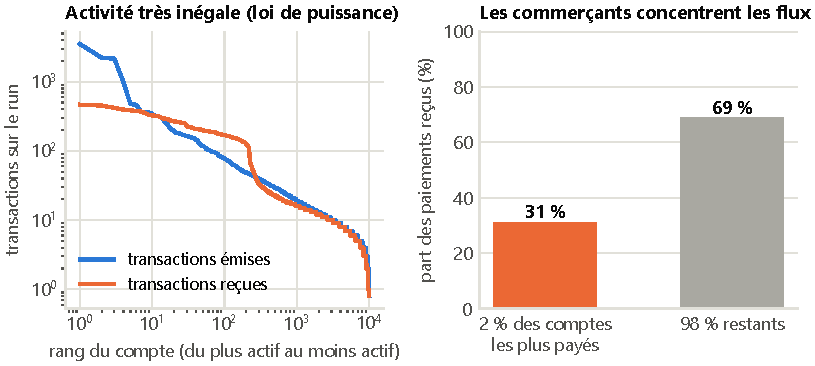
\includegraphics[width=\linewidth]{figures/activite_comptes.pdf}
\caption[Activité des comptes pendant le run]{Activité des 10\,000 comptes pendant le run d'évaluation :
quelques comptes concentrent l'essentiel des transactions (gauche, échelles logarithmiques) et
les 2\,\% de comptes les plus payés reçoivent près d'un tiers des paiements (droite).}
\label{fig:activite}
\end{figure}

Les montants dépendent du type d'opération : chaque type a un montant
médian propre et une dispersion log-normale (figure~\ref{fig:montants}). Le
seuil de 20\,000~MAD, au-dessus duquel le chemin lent construit son « graphe
des gros flux », ne retient qu'une petite minorité du trafic légitime.

\begin{figure}[htp]
\centering
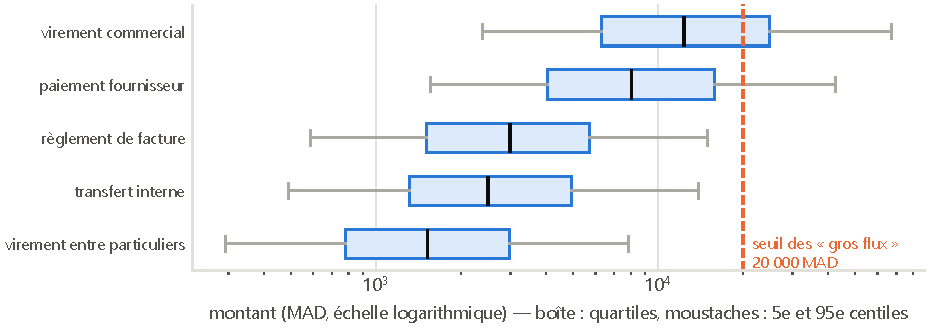
\includegraphics[width=\linewidth]{figures/montants_types.pdf}
\caption[Montants par type d'opération]{Montants par type d'opération (échantillon de 40\,000
transactions du run). Poids dans le trafic : particuliers 35\,\%, fournisseurs 20\,\%, factures 20\,\%,
commerciaux 15\,\%, internes 10\,\%.}
\label{fig:montants}
\end{figure}

\section{Les fraudes injectées}
Le producteur injecte à intervalle régulier l'une des cinq typologies du
chapitre~\ref{ch:etatart}, en choisissant des comptes « écrans » parmi le tiers
le moins actif de la population (tableau~\ref{tab:scenarios}). Les virements
d'une fraude sont étalés dans le temps et mêlés au trafic normal, comme dans
la réalité (figure~\ref{fig:scenarios}). Pour chaque fraude, le producteur
publie dans \fichier{ground-truth} son type, ses comptes, les identifiants de
ses transactions et son heure d'injection : c'est la \motcle{vérité terrain}
qui permet de calculer rappel et précision au chapitre~\ref{ch:resultats}.

\begin{table}[htp]
\centering\small
\begin{tabular}{@{}l>{\raggedright\arraybackslash}p{3.0cm}>{\raggedright\arraybackslash}p{3.3cm}>{\raggedright\arraybackslash}p{2.6cm}>{\raggedright\arraybackslash}p{2.5cm}@{}}
\toprule
\sffamily\bfseries Typologie & \sffamily\bfseries Comptes & \sffamily\bfseries Montants & \sffamily\bfseries Rythme & \sffamily\bfseries Signature\\
\midrule
{\color{cat1}\ico{F111}}~Carrousel & 3 sociétés & 40--250\,k MAD, $-$1 à 3\,\% par étape & 20--90~s entre virements & boucle fermée\\
{\color{cat3}\ico{F111}}~Cycle long & 4 ou 5 sociétés & idem & idem & boucle longue\\
{\color{cat5}\ico{F111}}~Compte mule & 8--14 émetteurs, 1 mule, 1 bénéficiaire & dépôts 2--9,8\,k ; retrait 90--97\,\% & dépôts toutes les 5--25~s & entonnoir puis vidage\\
{\color{cat4}\ico{F111}}~Scatter-gather & 1 source, 4--6 intermédiaires, 1 destination & 60--200\,k MAD répartis en parts égales & 15--60~s par relais & éventail puis regroupement\\
{\color{cat2}\ico{F111}}~Pivot & 1 pivot + 6 comptes & 3 carrousels de 60--150\,k & décalés de 10--40~s & 3 boucles, 1 compte commun\\
\bottomrule
\end{tabular}
\caption{Paramètres de génération des cinq typologies (\fichier{fraud/scenarios.py}).}
\label{tab:scenarios}
\end{table}

\begin{figure}[htp]
\centering
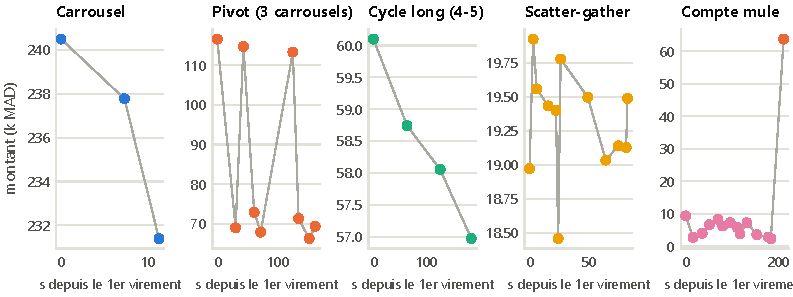
\includegraphics[width=\linewidth]{figures/scenarios_chronologie.pdf}
\caption[Chronologie de cinq fraudes réelles du run]{Chronologie d'une fraude de chaque type
injectée pendant le run : montant de chaque virement en fonction du temps écoulé depuis le premier.
On lit la commission du carrousel, les trois boucles imbriquées du pivot, la rafale de petits dépôts
de la mule suivie du retrait.}
\label{fig:scenarios}
\end{figure}

\section{Le run d'évaluation}
Toutes les figures de données de ce rapport, sauf mention contraire,
proviennent d'un même run de 42~minutes (figure~\ref{fig:trafic}) : 50
transactions par seconde, une fraude toutes les 30~secondes, après une
chauffe de 11~minutes sans fraude. Cette chauffe n'est pas un artifice : la
règle des comptes mules compare le rythme de dépôts d'un compte à son rythme
habituel, qu'il faut d'abord avoir observé.

\begin{figure}[htp]
\centering
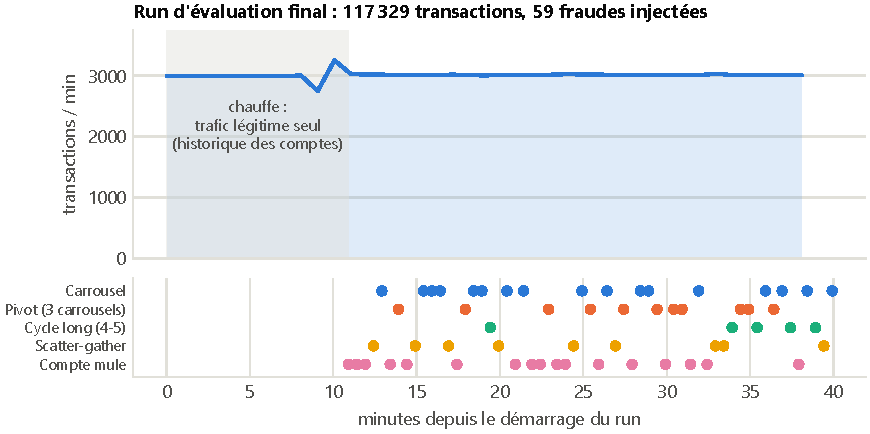
\includegraphics[width=\linewidth]{figures/trafic_run.pdf}
\caption[Trafic et fraudes injectées pendant le run d'évaluation]{Trafic et fraudes injectées pendant
le run d'évaluation. Les fraudes injectées dans les 8 dernières minutes ne comptent pas dans le
rappel, faute de temps pour être détectées : 42 fraudes sont évaluées.}
\label{fig:trafic}
\end{figure}

\section{Données imparfaites, comme en production}
Le producteur dégrade volontairement une petite partie du flux : 0,2\,\% des
messages arrivent en retard (la moitié de 30 à 100~s, l'autre moitié de 150
à 300~s, donc au-delà du watermark) et 0,05\,\% sont invalides. Le job doit
accepter les premiers, écarter les seconds, et isoler les messages invalides
dans une table de quarantaine sans jamais interrompre le flux
(figure~\ref{fig:qualite}).

\begin{figure}[htp]
\centering
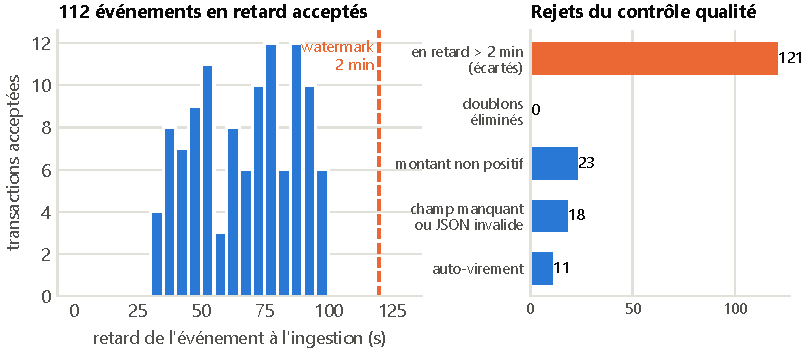
\includegraphics[width=\linewidth]{figures/qualite_donnees.pdf}
\caption[Contrôle qualité pendant le run]{Contrôle qualité pendant le run. À gauche, les événements en
retard de moins de 2~minutes sont intégrés au graphe. À droite, les 121 événements trop anciens sont
écartés par le watermark et les 52 messages invalides partent en quarantaine, avec leur motif.}
\label{fig:qualite}
\end{figure}

\aretenir{À retenir}{Le flux est réaliste (hubs, loi de puissance, retards, erreurs) et chaque fraude
injectée est connue avec précision. On peut donc \emph{mesurer} la détection plutôt que l'illustrer
sur quelques exemples choisis.}
